\section{Tribler}
	\label{scc:tribler}
	In this section an overview of Tribler and its components is presented. We describe the new beta version that uses anonymous tunnels in depth. Furthermore we look at what specific dependencies Tribler relies on.

	\subsection{What is Tribler?}
		Tribler is a fully decentralized peer-to-peer file sharing system developed by the Parallel and Distributed Systems group at Delft University of Technology. It has been in development for over 9 years and has a very mature and well-established code base. It allows users to search for and share files in a fully decentralized way. This decentralized nature of Tribler has several advantages over existing file sharing systems. The lack of a centralized component makes it very scalable and practically impossible to bring down.
		
		A new version of Tribler is currently in beta that includes a python implementation of a tor-like protocol. This enables users to share files anonymously and securely. By encrypting and routing traffic over a circuit of nodes, it ensures the communicating parties are oblivious of each other's virtual and physical location. More details about these anontunnels can be found in section \ref{sec:anonymoustunnels}.

	\subsection{M2Crypto}
		Tribler makes use of cryptographic functions to encrypt data and make their application secure. Security is a big issue in the world of peer-to-peer networks. Not only do we want anonymous downloads, we also want confidentiality and integrity of our data. Confidentiality means that unauthorized parties cannot see the exact content of the information. This could be achieved by encrypting the data. Integrity of the data means that the data is protected from being modified by other parties. Integrity can be achieved taking the hash of the data you receive and comparing it by taking the hash of the original message. If the hashes are not equal, the message has been modified. Confidentiality and integrity are important. When we are sending confidential data over the Internet, it would not be beneficial if everyone has access to the message and can read what is being send. Integrity can play a role when transferring money to another bank account: we do not want an adversary to temper with the amount of money that is being transferred.
		
		Some popular open source frameworks exists for these cryptographic tasks. A popular project is OpenSSL \cite{openssl}. OpenSSL implements the popular SSL and TLS protocols. These are cryptographic protocols that provides security when communicating over the internet. Besides that, OpenSSL provides libraries for various encryption and decryption protocols such as DES, RSA and RC4. OpenSSL also supports key exchange protocols such as Diffie-Hellman.
		
		OpenSSL is written in C. To use the OpenSSL libraries in Python, one could use pyopenssl \cite{pyopensslgithub}, a interface for OpenSSL or M2Crypto \cite{m2cryptogithub} (M2Crypto stands for 'Me Too Crypto'), an OpenSSL wrapper. Tribler makes use of the M2Crypto library. The old homepage of the M2Crypto project explains what M2Crypto is:
		
		\begin{quote}
		"M2Crypto is the most complete Python wrapper for OpenSSL featuring RSA, DSA, DH, HMACs, message digests, symmetric ciphers (including AES); SSL functionality to implement clients and servers; HTTPS extensions to Python's httplib, urllib, and xmlrpclib; unforgeable HMAC'ing AuthCookies for web session management; FTP/TLS client and server; S/MIME; ZServerSSL: A HTTPS server for Zope and ZSmime: An S/MIME messenger for Zope. M2Crypto can also be used to provide SSL for Twisted." \cite{m2crypto}
		\end{quote}
		
	\subsection{Dispersy}
		Dispersy \cite{zeilemaker2013dispersy} is a fully decentralized system for data bundle synchronization used by Tribler. The system is designed in such a way that it is capable of running in a challenging network environment. Such an environment is often characterized by:
		\begin{itemize}
			\item Nodes randomly joining and leaving.
			\item Delays in the network.
			\item Nodes having different networking speeds (Edge, 3G, WiFi).
			\item Nodes often being behind routers with Network Address Translating (NAT) firewalls.
		\end{itemize}
		
		All communication done by Dispersy uses UDP. Because up to 64\% of the internet is behind a NAT, they can use UDP firewall-NAT puncturing mechanisms\cite{zeilemaker2013dispersy}.
		
		In Dispersy, each node has a candidate list. A candidate list is a list of active connections within the node's overlay. A Dispersy node synchronizes in five steps:
		
		\begin{enumerate}
			\item First it selects a node from its candidate list.
			\item It then selects a range of bundles to synchronize.
			\item The node creates a Bloomfilter by hashing the selected bundles.
			\item Then the node sends the created Bloomfilter to the selected node.
			\item Finally, it pauses for a fixed interval to go back to step 1.
		\end{enumerate}
		
		The candidate list is divided into three sections: trusted nodes, nodes that have been successfully contacted in the past and nodes that have been connected in the past either trough an introduction-request or nodes that have been introduced.
		
		A Bloomfilter uses a hash area consisting of \emph{N} bits, initially all set to zero. For each item that needs to be stored in the Bloomfilter, \emph{K} distinct addresses are generated using a hash of the item. The bits addressed in the Bloomfilter are then set to one. To check if an item is part of a Bloomfilter, one only has to generate the hash of that item and check if the addresses that are generated by the hash are one in the Bloomfilter.
		
		After benchmarking Dispersy against Cassandra (the database system used by Facebook), they came to the conclusion that Dispersy performs better than Cassandra. By using Bloomfilters, Dispersy can scale to over 100,000 bundles to synchronize.
		
	\subsection{Anonymous tunnels}
	\label{sec:anonymoustunnels}
		Recently, the research team of Tribler started to work on the implementation of anonymous downloads. Pull request 525 on the Tribler Github page \cite{pullrequest525} is an experimental build of Tribler with the implementation of anonymous communications. The anonymous communication is achived by using a Tor-like protocol. This protocol has been implemented in Python and uses a three-hop circuit for anonymous communication. Note that Tribler does not use the Tor network, only a Tor-like protocol with UDP connections.
		
		The anonymous tunnels are implemented in the Python module \emph{Tribler.community.anontunnel}. Taking the code as reference, we now describe various details of the anonymous tunnels.
		
		\begin{itemize} 
			\item The circuit setup is using the Diffie-Hellman key exchange protocol to establish a secure connection. The M2Crypto library is used for the Diffie-Hellman protocol.
			\item The experimental code is using the Socks5 protocol for communication with other nodes. This code has been written by the Tribler team.
			\item Dispersy is used as a cache system to keep track of the outstanding PING and EXTEND requests and of candidates used in CREATE and CREATED requests.
			\item A circuit can be in four states: ready, extending, to be extended or broken.
			\item There are nine different messages that can be send amongst nodes: create, created, extend, extended, data, ping, pong, puncture and stats.
		\end{itemize}
		
		In order to test the anonymous connections and the download speed, a special anonymous tab has been built into Tribler. Clicking on this tab brings up a graph of the current anonymous network as a graph. It also logs the circuit events such as the extend or creation of a circuit. When enough anonymous proxies are online, a 50MB test download file should start to download.
	
		\begin{figure*}[!t]
			\centering
			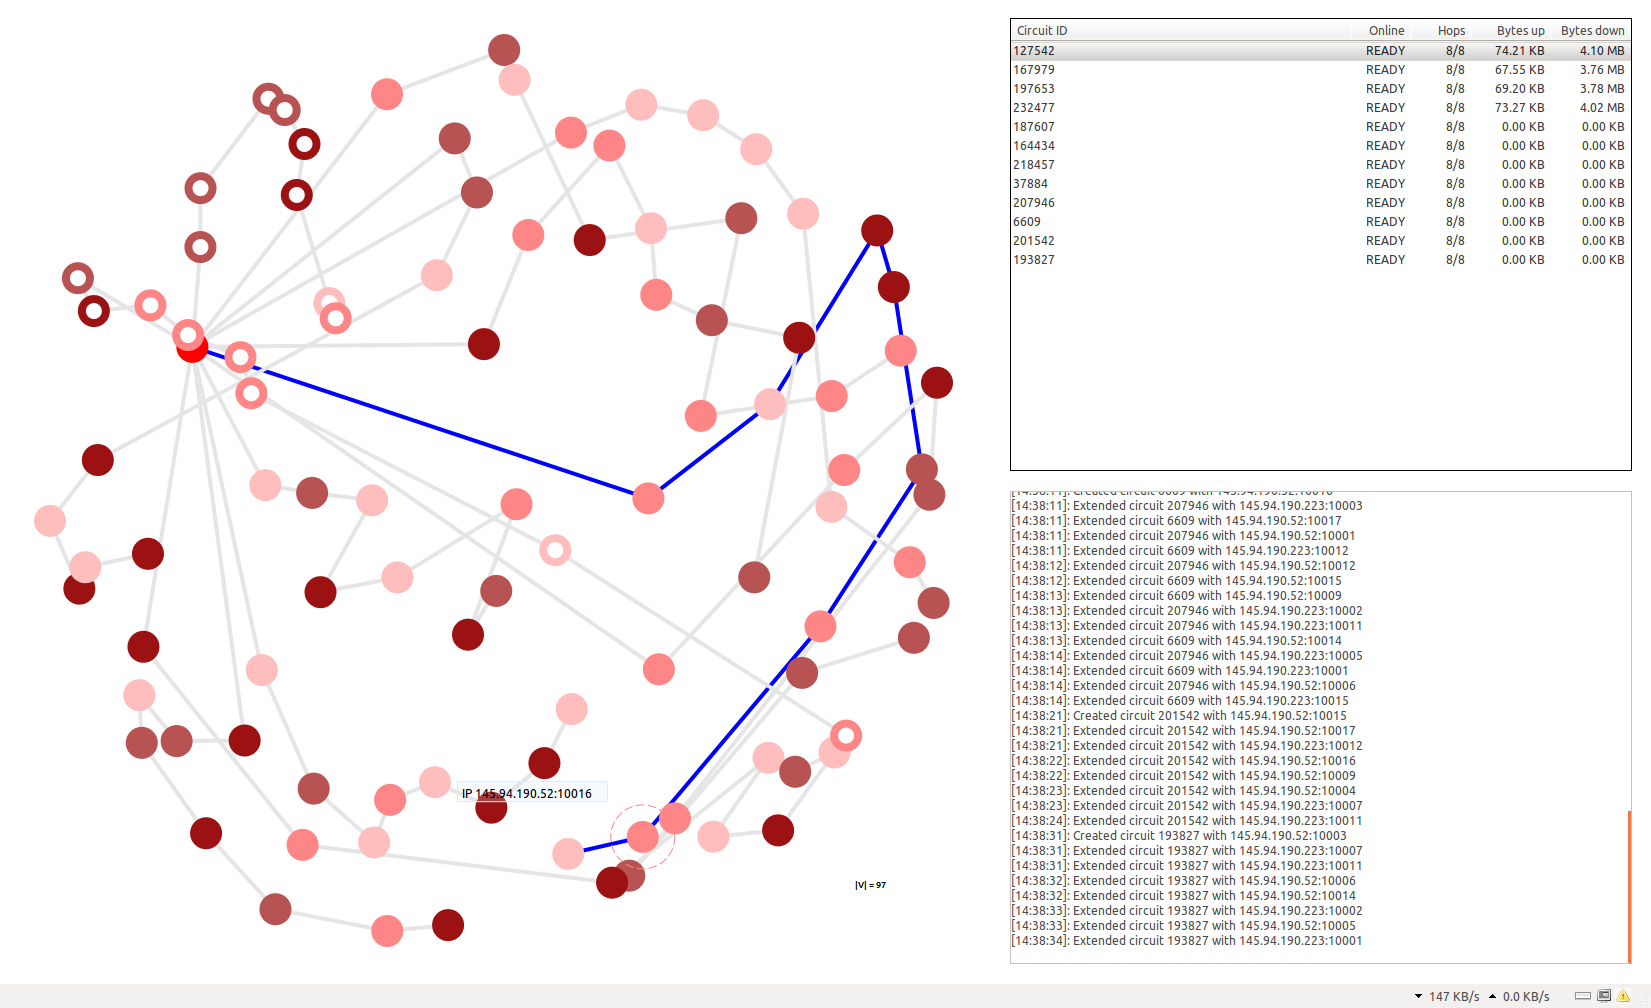
\includegraphics[width=0.8\textwidth]{prior-work/8hop.png}
			\caption{The graphical user interface in Tribler that shows the anonymous network.}
			\label{fig:anon_downloads}
		\end{figure*}